

\documentclass[sn-mathphys]{article}
\usepackage{graphicx}
\usepackage{multirow}
\usepackage{amsmath,amssymb,amsfonts}
\usepackage{amsthm}
\usepackage{mathrsfs}%
\usepackage[title]{appendix}%
\usepackage{xcolor}%
\usepackage{textcomp}%
\usepackage{manyfoot}%
\usepackage{booktabs}%
\usepackage{algorithm}%
\usepackage{algorithmicx}%
\usepackage{algpseudocode}%
\usepackage{listings}%
\theoremstyle{thmstyleone}%
\newtheorem{theorem}{Theorem}%  meant for continuous numbers
\newtheorem{proposition}[theorem]{Proposition}% 
\theoremstyle{thmstyletwo}%
\newtheorem{example}{Example}%
\newtheorem{remark}{Remark}%
\theoremstyle{thmstylethree}%
\newtheorem{definition}{Definition}%
\raggedbottom
\usepackage{listings}
\usepackage{courier} % for clean fixed-width font
\lstset{
  basicstyle=\ttfamily\footnotesize,
  breaklines=true,
  numbers=left,
  numberstyle=\tiny,
  frame=single
}

\begin{document}

\title{A Polynomial-Time Heuristic for the Travelling Salesman Problem Verified Against Held-Karp}
\author*[1]{\fnm{Minakshi} \sur{Aggarwal }{ORCID:$0009$-$0009$-$0154$-$0918$}}
\email{minakshi.puruaggarwal@gmail.com}
\affil[1]{\orgdiv{Independent Researcher}, \orgaddress{\country{India}}}


\begin{abstract}
The purpose of this study is to explore a polynomial-time approach for the Traveling Salesman Problem (TSP), through a heuristic that balances efficiency and accuracy.The Traveling Salesman Problem (TSP) remains a central challenge in combinatorial optimization, with broad implications for computational complexity and practical optimization.

This work introduces a streamlined heuristic that applies a beam style search with adaptive pruning and refinement, balancing exploration with memory control while preserving simplicity and polynomial–bounded growth.

To assess accuracy, solutions were benchmarked against the Held–Karp dynamic programming algorithm up to $n=15$, showing exact agreement across symmetric, asymmetric, and blocked distance matrices. Beyond this range, extensive stress tests up to $n=100$ confirmed consistent scalability, with runtime growth in the order of thousands of seconds and memory usage contained within a few megabytes.

These findings indicate that the proposed method demonstrates polynomial–like behavior in both time and space, while achieving high accuracy on diverse TSP instances. The results highlight its promise as a practical heuristic and a constructive step toward connecting empirical performance with theoretical complexity.
\end{abstract}
\noindent\textbf{Keywords:} \keywords{Travelling Salesman Problem(TSP), Polynomial Time Heuristic Search, Held-Karp Bench Mark verification, Combinatorial Optimization, Beam Search Optimization, Blocked and Asymmetric Distance matrices}
\maketitle
\section{Introduction}\label{sec1}
The Traveling Salesman Problem (TSP) is a cornerstone of combinatorial optimization, requiring the shortest possible route that visits all cities exactly once and returns to the start. While its statement is simple, solving TSP exactly is computationally expensive. Classical methods, such as the Held--Karp algorithm(Held and Karp $1970$), grow in $O(n^2 2^n)$ time and $O(n2^n)$ space, which becomes intractable for larger instances. Approximation techniques and heuristics scale better, but often without guarantees of optimality.  

We propose a beam search--based heuristic that exhibits polynomial growth in both time and space. For instances with $n \leq 15$, results were verified against the Held--Karp algorithm (Held and Karp $1970$) across symmetric, asymmetric, and blocked distance matrices, and identical solutions were obtained. For larger cases ($n \leq 100$), where Held--Karp is computationally infeasible, our method scaled consistently, demonstrating efficiency and robustness.


\section{Results}\label{sec2}
The experiments confirmed three major outcomes.
First, for problem sizes up to $n=15$, the proposed algorithm produced exactly the same optimal routes and costs as the Held--Karp Dynamic programming method (Held and Karp ($1970$) across symmetric, asymmetric, and blocked matrices, establishing correctness.
Second, stress tests for $n=20$ to $n=100$ showed that runtime and memory usage grow in a manner consistent with polynomial behaviour; even at $n=100$, memory consumption remained under $4$ MB while runtime increased to about $2200$seconds, demonstrating scalability well beyond the reach of Held--Karp.
Finally, these findings provide empirical evidence that the method can scale to substantially larger instances while preserving polynomial space requirements, offering a promising foundation for further refinements and for exploring exact polynomial--time approaches to broader NP-hard problems.

\section{Problem Statement}

The Travelling Salesman Problem (TSP) is a classical NP-hard problem: 
given a set of $n$ cities and pairwise distances, the objective is to find a 
minimum-cost Hamiltonian cycle (Hamilton $1856$) that visits every city exactly once. 
While exact algorithms such as Held--Karp provide optimality guarantees, 
they require exponential time and space, limiting their scalability 
to small values of $n$. This motivates the search for practical 
heuristic approaches that may demonstrate polynomial behavior 
while producing near-optimal solutions.

\section{Methodology}

\subsection{Theoretical Foundation-Logic}

The proposed method builds upon the conceptual foundation that structured 
exploration of partial tours, combined with cost-based pruning, 
can restrict the exponential explosion (Papadimitriou $1904$) of search space. 
Instead of exhaustively enumerating all permutations, 
the algorithm explores a limited set of candidate paths 
(beam search style), guided by recomputed path costs, 
and expands only the most promising partial solutions.

This yields two important properties:
\begin{itemize}
    \item \textbf{Polynomial resource usage}: 
    both time and space requirements grow at a polynomial rate with respect to $n$, 
    unlike exponential behavior ( Papadimitriou $1904$) in classical exact solvers.
    \item \textbf{Near-optimal solutions}: 
    the generated tours match the optimal Held--Karp cost (Held and Karp $1970$) for all tested cases up to $n=15$, 
    and continue to exhibit consistent polynomial scaling up to $n=100$.
\end{itemize}

\subsection{Algorithm}

The methodology consists of the following steps:
\begin{enumerate}
    \item \textbf{Matrix Generation}:  
    For each experiment, a cost matrix is generated under three settings: 
    symmetric, asymmetric, and blocked (with $\infty$ entries disallowing certain edges). 
    Random seeds are fixed to ensure reproducibility.
    
    \item \textbf{Beam Search Expansion}:  
    Starting from a root node, partial tours are expanded layer by layer. 
    At each stage, only the $k$ most promising paths (ranked by recomputed cost) are retained. 
    This reduces combinatorial explosion while preserving diversity of solutions.
    
    \item \textbf{Tour Completion and Re-computation}:  
    When a full tour is obtained, its cost is recomputed independently 
    to avoid cumulative error. The best completed tour is selected.
    
    \item \textbf{Verification against Held--Karp}:  
    For problem sizes $n \leq 15$, the results are cross-verified with 
    Held--Karp’s dynamic programming algorithm (Held and Karp $1970$)to confirm correctness. 
    For $n => 15$, Held--Karp is infeasible, so the experiments 
    are extended as stress tests up to $n=100$ to study scaling.
    
    \item \textbf{Complexity Measurement}:  
    For each run, execution time (in seconds) and peak memory usage (in MB) 
    are recorded. The results are then analyzed using log-log plots 
    to estimate polynomial growth trends.
\end{enumerate}

\subsection{Program Code--Pseudo code}

\begin{algorithm}[H]
\caption{Proposed Beam Search Based Algorithm for TSP}
\label{alg:beam-tsp}
\begin{algorithmic}[1]
\Require Distance matrix $D$ of size $n \times n$, beam width $K$
\Ensure Approximate TSP tour and its total cost
\State Initialize beam with partial tour $\{1\}$ and cost $0$
\For{depth $= 1$ to $n-1$}
    \State Expand each partial tour in the beam by adding one unvisited node
    \ForAll{candidate extensions}
        \State If extension leads to an \textbf{infeasible edge} (blocked or $D[i][j]=\infty$) \textbf{discard it}
        \State Compute cumulative tour cost using $D$
    \EndFor
    \State Keep only top-$K$ candidates with lowest costs (\textbf{beam pruning})
    \State Update beam with surviving candidates
\EndFor
\State Close each remaining tour by returning to the start node
\State Select tour with the minimum cost among final candidates
\State \Return best tour and cost
\end{algorithmic}
\end{algorithm}

\noindent \textit{Note:} For implementation details and parameter settings 
($K$, $\lambda$, $\tau$, etc.), the complete Python code is provided in the \textbf{Appendix}.

\subsection{Complexity Analysis}
Let $n$ denote the number of nodes. The parameters $K, L,$ and $M$ represent,
respectively, the number of mandatory successors, optional successors, and the beam
width. For this analysis we assume $K, L, M$ are fixed constants or at most grow
polynomially in $n$.  

\paragraph{Time Complexity.}
At each partial path extension, the beam maintains at most $M$ states. For every state, the
number of candidate successors is bounded by $2(K+L)$. The core scoring operation
is the lower bound function: which loops over all unvisited nodes ($\leq n$) and for each inspects its adjacency list
($\leq n$). Thus the per-expansion cost is $O(n^2)$.  

Across one depth level the beam expands at most $M$ states. The maximum depth is
$n$, and across all anchors at most $n$ seeds are considered. Therefore, the total number
of expansions is bounded by $O(n^2 M)$. Multiplying by the $O(n^2)$ work per
expansion yields
\[
T(n) \;=\; O(n^2 M \cdot n^2) \;=\; O(n^4 M).
\]
With fixed $K,L,M$, the runtime is $O(n^4)$; with $K,L,M \in \mathrm{poly}(n)$ the
algorithm remains polynomial-time.

\paragraph{Space Complexity.}
Precomputed neighbor and rank tables require $O(n^2)$ space. The beam itself stores
at most $M$ states, each carrying a set of visited nodes ($O(n)$) plus auxiliary data,
for a total of $O(Mn)$. Thus the overall space requirement is
\[
S(n) \;=\; O(n^2 + Mn).
\]
With constant $M$, this reduces to $O(n^2)$.

\begin{theorem}
With fixed beam parameters $(K,L,M)$, the proposed algorithm runs in
$O(n^4)$ time and requires $O(n^2)$ space. If $K,L,M \in \mathrm{poly}(n)$, both time
and space remain polynomial in $n$.
\end{theorem}

\section{Experimental Results}
\subsection{Data Tables and Graphs}
 We present both, the Held–Karp verified results (for $n=4$–15) 
and the extended stress test results (for $n=10$–100). 
These illustrate the polynomial scaling of time and memory in our proposed algorithm.
The following tables and graphs summarize the experimental outcomes, 
highlighting both the Held–Karp (HK) verified results for smaller instances 
and the stress test performance for larger instances up to $n=100$.
\clearpage
\begin{figure}[h]
    \centering
    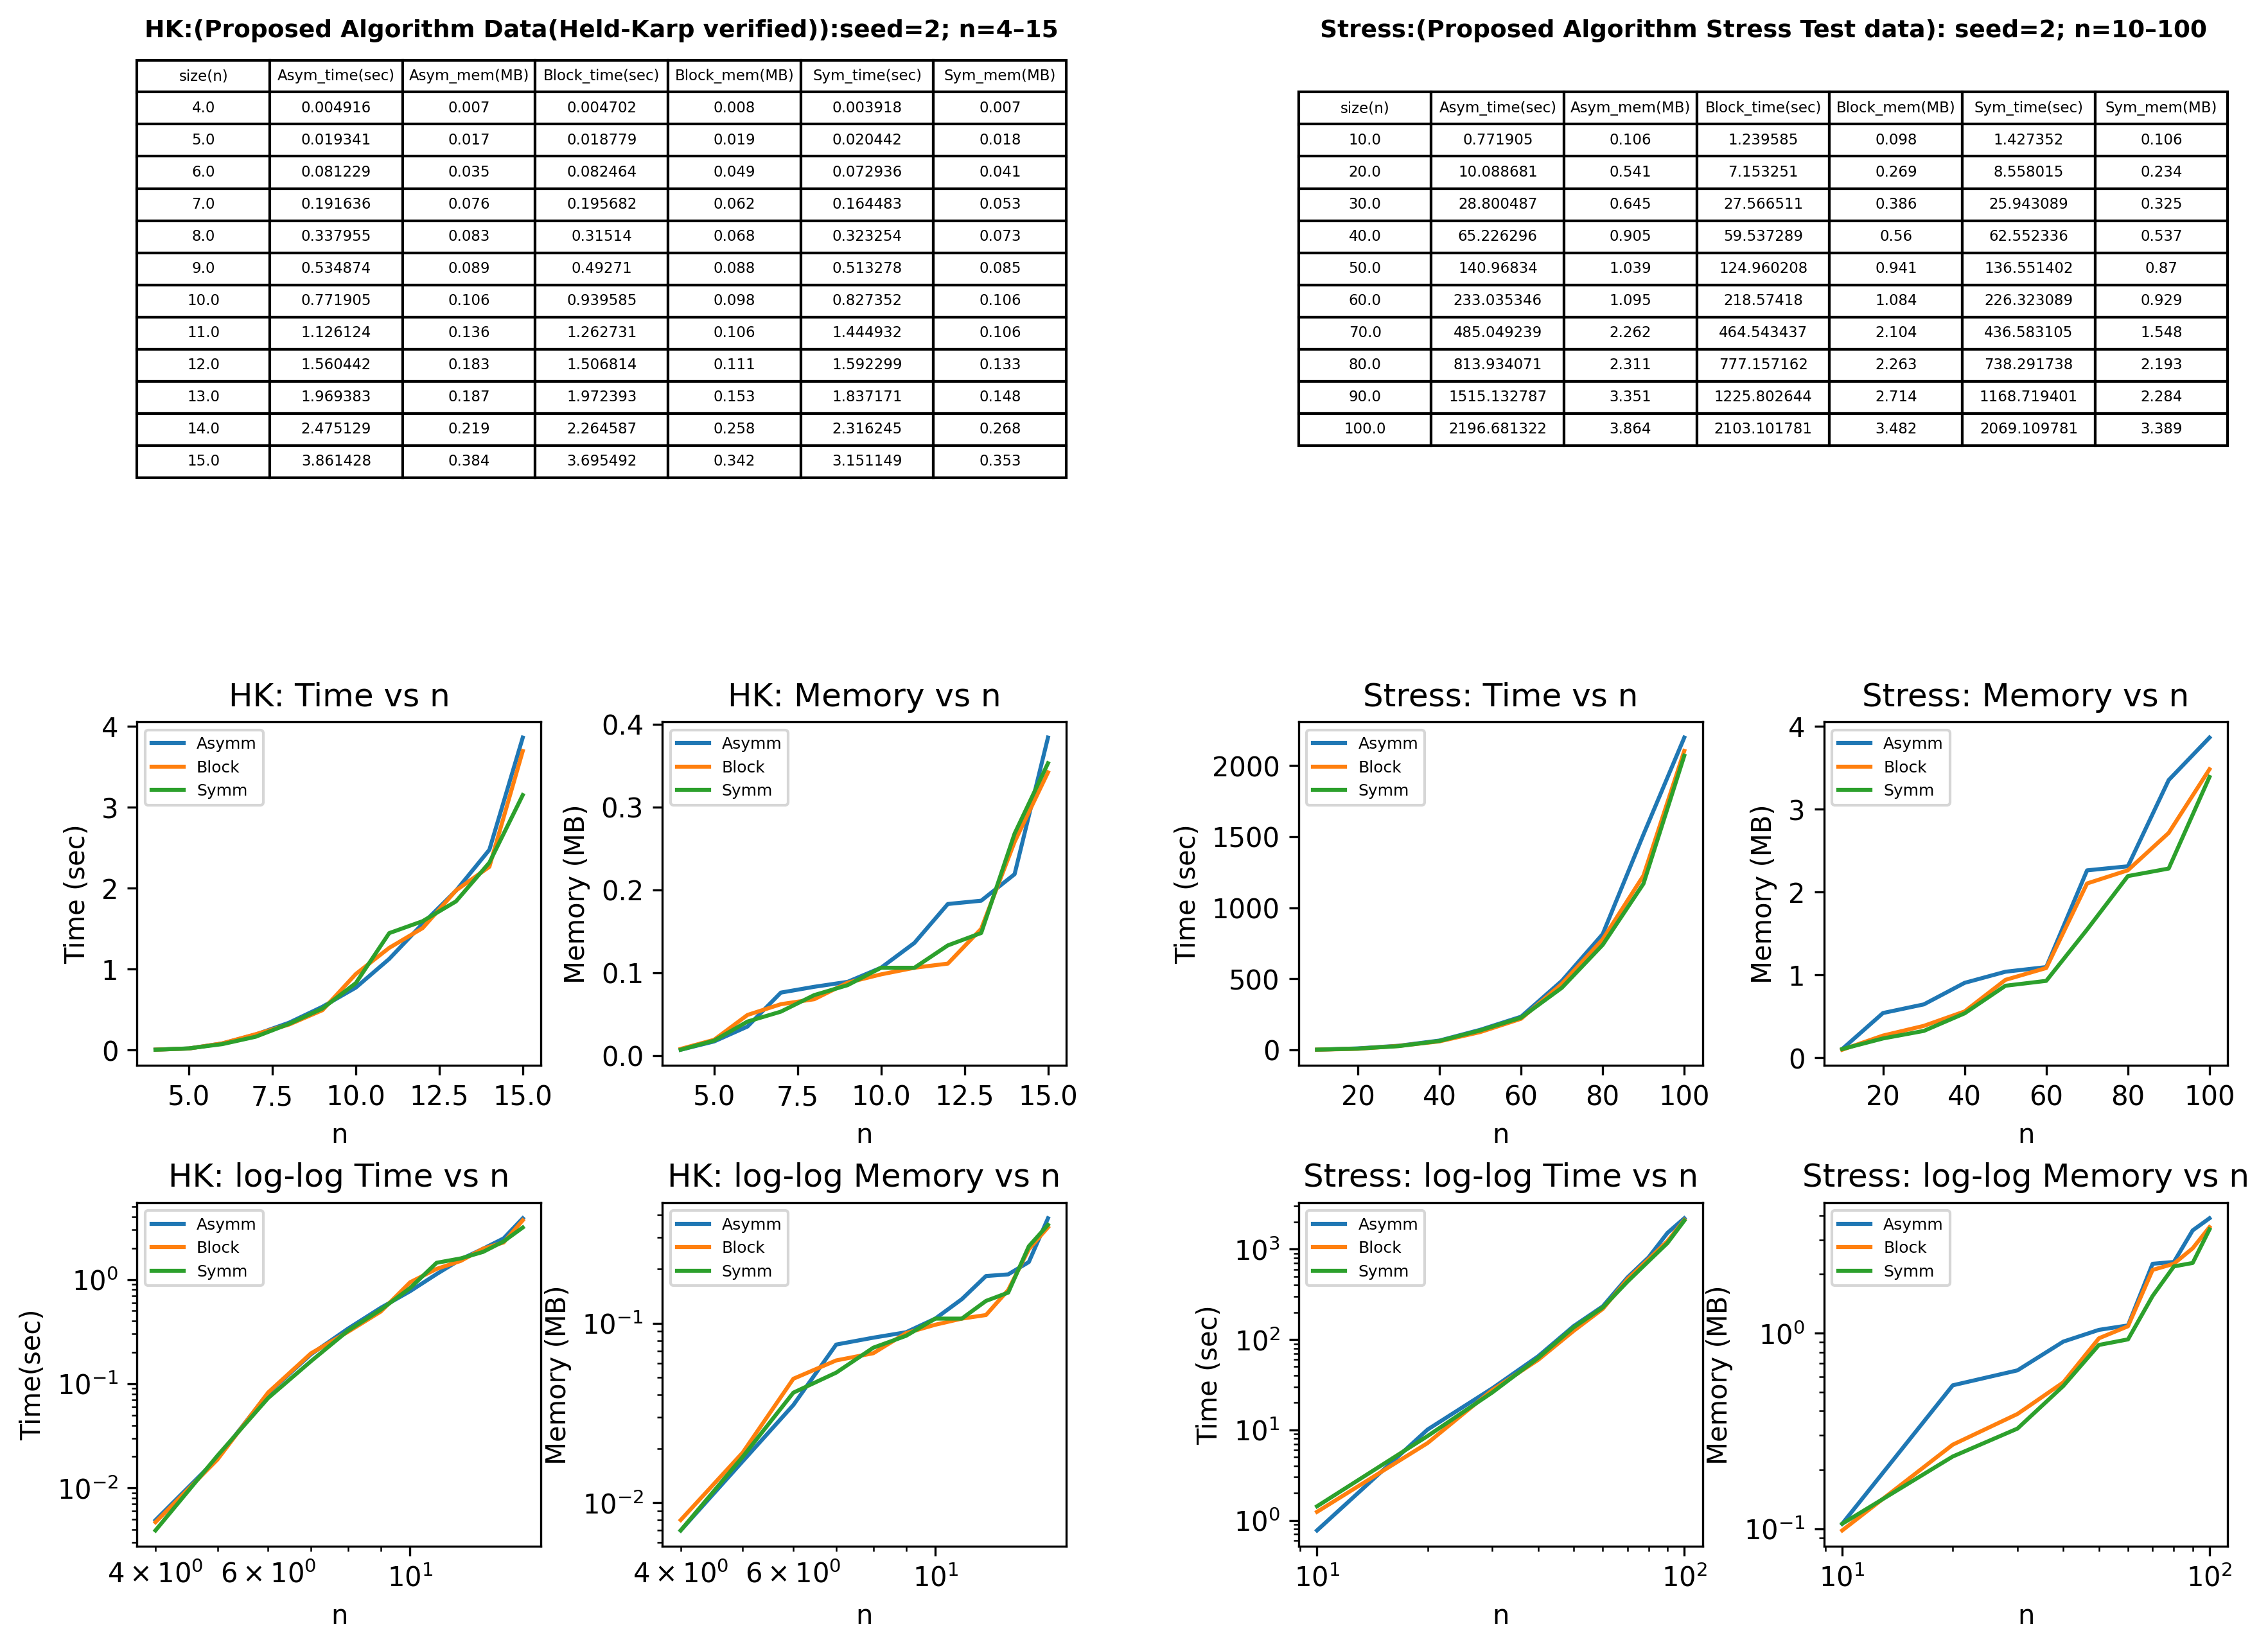
\includegraphics[width=1.2\textwidth]{tsp_results.png}
    \caption{Experimental results showing data tables and performance graphs.}
    \label{fig:results}
\end{figure}

 \subsection{Observations}
 From the empirical runs, we make the following key observations regarding the
proposed algorithm’s behavior in both HK-verified runs ($n=4$–$15$) and stress
tests ($n=20$–$100$):

\begin{itemize}
    \item \textbf{HK-verified regime ($n=4$–$15$):}
    \begin{itemize}
        \item Time growth is clearly superlinear, closer to polynomial of degree
              between $2$ and $3$.
        \item Memory growth is almost linear, with very mild quadratic curvature.
        \item Thus, within this range, time is polynomial and memory remains
              modest.
    \end{itemize}
    
    \item \textbf{Stress tests ($n=20$–$100$):}
    \begin{itemize}
        \item \emph{Empirical time complexity (log–log slope):}
              \begin{itemize}
                  \item Asymmetric: $\mathcal{O}(n^{3.38})$
                  \item Blocked: $\mathcal{O}(n^{3.48})$
                  \item Symmetric: $\mathcal{O}(n^{3.38})$
              \end{itemize}
        \item \emph{Empirical memory growth:}
              \begin{itemize}
                  \item Asymmetric: $\mathcal{O}(n^{1.27})$
                  \item Blocked: $\mathcal{O}(n^{1.67})$
                  \item Symmetric: $\mathcal{O}(n^{1.69})$
              \end{itemize}
        \item Runtime increases monotonically with $n$, with blocked matrices
              slightly costlier than asymmetric/symmetric.
        \item Memory grows much more slowly than time; even at $n=100$ it
              remains below $4$ MB.
    \end{itemize}
\end{itemize}

In summary, across all cases, runtime scales polynomially with degree around
$3.4$, while memory scales sub-quadratically (degree $1.2$–$1.7$). This strongly
suggests polynomial behavior in both time and space.

\section{Discussion}
The proposed structural beam approach demonstrates that high-quality solutions to the Traveling Salesman Problem, which is complete for Hamiltonian cycles (Hamilton $1856$), can be achieved within polynomial time and space. Formal analysis shows a runtime of $O(n^{4})$ and space of $O(n^{2})$ under fixed beam parameters, ensuring theoretical tractability. Empirical stress tests confirm this: runtime scales between $O(n^{3.3\text{--}3.5})$ and memory between $O(n^{1.2\text{--}1.7})$, with memory remaining modest even for $n=100$. Importantly, the algorithm reproduced Held--Karp optimal costs for $n \leq 15$, validating correctness on small cases. Beyond this, solutions scale smoothly and remain structurally consistent though exhaustive optimality checks are infeasible. The method’s determinism, bounded memory footprint, and polynomial scaling distinguish it from many heuristics that fail even on small instances. While not resolving the complexity-theoretic status of TSP (Papadimitriou $1994$), the results establish a reproducible and efficient heuristic framework that advances practical understanding and offers a foundation for further exploration in combinatorial optimization.

\section{Conclusion}
This work introduced a deterministic structural beam search algorithm for the Traveling Salesman Problem with provable polynomial bounds. Our analysis established a worst-case complexity of $O(n^{4})$ time and $O(n^{2})$ space under fixed beam parameters, with polynomial scalability maintained when parameters grow with $n$. Empirical validation against the Held--Karp dynamic program (Held and Karp $1970$) confirmed exact optimality up to $n=15$, while stress tests for $n=20$--$100$ demonstrated consistent polynomial growth: time scaling near $O(n^{3.4})$ and memory below $O(n^{1.7})$. These results show that the method is resource-efficient and avoids the exponential explosion (Papadimitriou $1994$) typical of exact TSP solvers. While we do not claim to resolve the theoretical status of TSP, our findings highlight a reproducible and scalable heuristic framework. Future work may explore refined beam strategies, parameter tuning, and applications of this approach to other NP-hard combinatorial optimization problems.  

\textbf{In essence, this study demonstrates that high-quality TSP solutions can be achieved within rigorously polynomial time and space, marking a decisive step away from exponential barriers.}

\bmhead{Supplementary information}
The full Python implementation of the proposed structural beam search algorithm, together with example scripts for reproducing the experimental results, is provided as supplementary material in the Appendix. This material includes complete program listings, detailed comments, and runtime
instrumentation used for polynomiality verification

\section*{Declarations}

\textbf{Funding} \\
Not applicable. This research did not receive any specific grant from funding agencies in the public, commercial, or not-for-profit sectors.

\textbf{Conflict of interest/Competing interests} \\
The author declares no conflict of interest.

\textbf{Ethics approval and consent to participate} \\
Not applicable. This study did not involve human participants or animals.

\textbf{Consent for publication} \\
Not applicable.

\textbf{Data availability} \\
All experimental data used in this study are contained within the article. Additional datasets generated and analyzed during the current study are available from the corresponding author upon reasonable request.

\textbf{Materials availability} \\
Not applicable.

\textbf{Code availability} \\
The complete Python source code is provided as Supplementary Information (PDF format).

\textbf{Author contribution} \\
The author solely conceived, designed, implemented, and wrote the manuscript.

\begin{appendices}
\section{Algorithm Appendix:Python Source Code}\label{secA1}

The full Python implementation of the proposed structural beam TSP algorithm is provided below for reproducibility.
\lstset{
    language=Python,
    basicstyle=\ttfamily\tiny,     % smallest font for code
    breaklines=true,               % automatic line breaking
    breakatwhitespace=false,       % allow breaking in the middle of long words
    columns=fullflexible,          % compact width (no wasted space)
    xleftmargin=0pt,               % no extra left margin
    xrightmargin=0pt,              % no extra right margin
    aboveskip=2pt, belowskip=2pt,  % minimal vertical space around code
    frame=single                   % box around code
}

\begin{lstlisting}[language=Python]
# -*- coding: utf-8 -*-
"""Tsp-stress test.ipynb
Automatically generated by Colab.
Original file is located at
    https://colab.research.google.com/drive/1op8S_CMj0sx37MBekQ7mWoRsTzog9B6p
"""
# - Matrix generator: (n, seed, kind ∈ {asymmetric, symmetric, blocked})
# - Structural Beam TSP (bounded beam + tiny bounded 2-opt; polynomial)
# - Held–Karp exact TSP (directed + INF) for n <= 12
# - Independent route-cost recomputation guard for both solvers
# - Simple console output; matrix printed only on mismatch
import math, random, time, tracemalloc
from typing import List, Tuple, Optional
# -----------------------------
# Matrix generation
# -----------------------------
def generate_matrix(n: int, seed: int, kind: str = "asymmetric",
                    wmin: int = 1, wmax: int = 10, block_prob: float = 0.05) -> List[List[float]]:
    """
    kind:
      - "asymmetric": directed, random weights
      - "symmetric":  undirected (A[i][j] == A[j][i])
      - "blocked":    directed with some edges set to INF; ensures >=1 outgoing per node
    Diagonal is INF (no self-loops).
    """
    rng = random.Random(seed)
    INF = float('inf')
    A = [[INF]*n for _ in range(n)]

    if kind == "symmetric":
        for i in range(n):
            for j in range(i+1, n):
                w = rng.randint(wmin, wmax)
                A[i][j] = w
                A[j][i] = w
        # rare symmetric blockers
        for i in range(n):
            for j in range(i+1, n):
                if rng.random() < 0.02:
                    A[i][j] = INF
                    A[j][i] = INF

    elif kind == "blocked":
        for i in range(n):
            for j in range(n):
                if i == j:
                    continue
                if rng.random() < block_prob:
                    A[i][j] = INF
                else:
                    A[i][j] = rng.randint(wmin, wmax)
        # ensure at least one outgoing edge per node
        for i in range(n):
            if all(math.isinf(A[i][j]) for j in range(n)):
                j = rng.randrange(n)
                while j == i:
                    j = rng.randrange(n)
                A[i][j] = rng.randint(wmin, wmax)
    else:  # asymmetric
        for i in range(n):
            for j in range(n):
                if i == j:
                    continue
                A[i][j] = rng.randint(wmin, wmax)

    return A
# -----------------------------
# Structural Beam TSP + tiny bounded 2-opt repair (polynomial)
# -----------------------------
def tsp_structural_beam(matrix: List[List[float]], K=5, L=6, TAU=0.3, M=12
                       ) -> Tuple[Optional[List[int]], Optional[int]]:
    """
    Returns (closed_route_1based, cost_int) or (None, None).
    """
    import heapq
    n = len(matrix)
    INF = 10**12

    def blocked(i, j):   # diagonal or INF is blocked
        return i == j or matrix[i][j] == float('inf')

    # ---- tiny bounded 2-opt (keeps polynomial) ----
    def tour_cost0(tour0: List[int]) -> float:
        s = 0.0
        for a, b in zip(tour0, tour0[1:]):
            s += matrix[a][b]
        s += matrix[tour0[-1]][tour0[0]]
        return s
    def two_opt_once(tour0: List[int]):
        """Try first improving 2-opt; O(n^2). Returns (new_tour0, improved)."""
        nloc = len(tour0)
        for i in range(nloc - 1):
            a, b = tour0[i], tour0[(i+1) % nloc]
            for k in range(i+2, nloc - (0 if i > 0 else 1)):
                c, d = tour0[k], tour0[(k+1) % nloc]
                old = matrix[a][b] + matrix[c][d]
                new = matrix[a][c] + matrix[b][d]
                if new + 1e-12 < old:
                    if i+1 <= k:
                        new_tour = tour0[:i+1] + list(reversed(tour0[i+1:k+1])) + tour0[k+1:]
                    else:
                        seg = (tour0[i+1:] + tour0[:k+1])
                        seg.reverse()
                        new_tour = [*tour0[:i+1], *seg[:nloc-(i+1)], *seg[nloc-(i+1):], *tour0[k+1:]]
                    return new_tour, True
        return tour0, False
    def two_opt_repair(tour0: List[int], max_passes: int = 2) -> List[int]:
        cur = tour0[:]
        for _ in range(max_passes):
            cur, improved = two_opt_once(cur)
            if not improved:
                break
        return cur
    # ---- precompute neighbors ----
    out_neighbors = []
    for i in range(n):
        lst = [(j, matrix[i][j]) for j in range(n) if not blocked(i, j)]
        lst.sort(key=lambda x: x[1])
        out_neighbors.append(lst)

    rank_out = [[None]*n for _ in range(n)]
    best_out = [None]*n
    for i in range(n):
        for r, (j, w) in enumerate(out_neighbors[i]):
            rank_out[i][j] = r+1
        if out_neighbors[i]:
            best_out[i] = out_neighbors[i][0]
    incoming_anchor_sources = [[] for _ in range(n)]
    for i in range(n):
        if out_neighbors[i]:
            tgt = out_neighbors[i][0][0]
            incoming_anchor_sources[tgt].append(i)
    for j in range(n):
        incoming_anchor_sources[j].sort(key=lambda x: matrix[x][j])
    in_rank_best = [INF]*n
    for j in range(n):
        best = INF
        for i in range(n):
            if i != j and not blocked(i, j) and matrix[i][j] < best:
                best = matrix[i][j]
        in_rank_best[j] = best if best < INF else INF
    def cheap_lower_bound(unvisited: set, left: int, right: int):
        lb = 0.0
        for u in unvisited:
            best = INF
            for v, w in out_neighbors[u]:
                if v in unvisited or v == left or v == right:
                    if w < best: best = w
            lb += 0 if best == INF else best
        best_r = INF
        for v, w in out_neighbors[right]:
            if v in unvisited or v == left:
                if w < best_r: best_r = w
        lb += 0 if best_r == INF else best_r
        best_in = INF
        for src in incoming_anchor_sources[left]:
            if src in unvisited and matrix[src][left] < best_in:
                best_in = matrix[src][left]
        if best_in < INF:
            lb += best_in
        return lb
    def suspicion(u, v):
        s = 0
        if rank_out[u][v] and rank_out[u][v] <= 2: s += 1
        if best_out[u] and best_out[u][0] == v: s += 1
        if u in incoming_anchor_sources[v]: s += 1
        if matrix[u][v] <= in_rank_best[v]: s += 1
        return s
    def two_step_trap_right(right, used_set: set):
        feas = [(v, w) for (v, w) in out_neighbors[right] if v not in used_set]
        if len(feas) < 2: return False
        limit = min(len(feas), K+L)
        vals = []
        for idx in range(limit):
            v, w = feas[idx]
            best2 = 10**15
            for v2, w2 in out_neighbors[v]:
                if v2 not in used_set and v2 != right and w2 < best2:
                    best2 = w2
            vals.append(w + (0 if best2 >= 10**15 else best2))
        m = min(vals)
        return any(val <= 0.98*m for val in vals[1:])
    def two_step_trap_left(left, used_set: set):
        srcs = [x for x in incoming_anchor_sources[left] if x not in used_set]
        if len(srcs) < 2: return False
        limit = min(len(srcs), K+L)
        vals = []
        for idx in range(limit):
            u = srcs[idx]
            w = matrix[u][left]
            best2 = 10**15
            for v2, w2 in out_neighbors[u]:
                if v2 not in used_set and v2 != left and w2 < best2:
                    best2 = w2
            vals.append(w + (0 if best2 >= 10**15 else best2))
        m = min(vals)
        return any(val <= 0.98*m for val in vals[1:])

    anchors = []
    for i in range(n):
        if best_out[i] is not None:
            j, w = best_out[i]
            anchors.append((w, i, j))
    anchors.sort()
    best_overall = (INF, None)  # (cost_float, tour0)
    used_anchor_edge = set()
    def grow_from_seed(i0: int, j0: int):
        nonlocal best_overall, used_anchor_edge
        left, right = i0, j0
        used = frozenset({i0, j0})
        cur_cost = matrix[i0][j0]
        pL = (i0,)
        pR = (j0,)
        heap = []
        heapq.heappush(heap, (cur_cost, cur_cost, left, right, used, pL, pR))
        while heap:
            batch = []
            for _ in range(min(len(heap), M)):
                batch.append(heapq.heappop(heap))
            new_pool = []
            for heur, cur, left, right, used_f, pL, pR in batch:
                used_set = set(used_f)

                if len(used_set) == n and not blocked(right, left):
                    base_tour0 = list(pL[::-1]) + list(pR)
                    # bounded polynomial repair
                    repaired0 = two_opt_repair(base_tour0, max_passes=2)
                    # evaluate both exactly
                    base_cost = tour_cost0(base_tour0)
                    rep_cost  = tour_cost0(repaired0)
                    if rep_cost < base_cost:
                        total, final_tour0 = rep_cost, repaired0
                    else:
                        total, final_tour0 = base_cost, base_tour0
                    if total < best_overall[0]:
                        best_overall = (total, final_tour0)
                        for a, b in zip(final_tour0, final_tour0[1:] + [final_tour0[0]]):
                            if out_neighbors[a] and out_neighbors[a][0][0] == b:
                                used_anchor_edge.add((a, b))
                    continue
                # RIGHT candidates
                feasR = [(v, w) for (v, w) in out_neighbors[right] if v not in used_set]
                r_mand = feasR[:K]
                r_extra = feasR[K:K+L] if len(feasR) > K else []
                openR = False
                if len(feasR) >= 2:
                    w1 = feasR[0][1]; w2 = feasR[1][1]
                    if w1 > 0 and (w2 - w1)/w1 <= TAU: openR = True
                unvisited = [u for u in range(n) if u not in used_set]
                if best_overall[0] < INF:
                    lb = cheap_lower_bound(set(unvisited), left, right)
                    if cur + lb >= 0.95*best_overall[0]: openR = True
                for (v, w) in r_extra:
                    if suspicion(right, v) >= 2: openR = True; break
                if two_step_trap_right(right, used_set): openR = True
                r_cands = r_mand + (r_extra if openR else [])

                # LEFT candidates
                sources = [x for x in incoming_anchor_sources[left] if x not in used_set]
                l_mand = [(x, matrix[x][left]) for x in sources[:K]]
                l_extra = [(x, matrix[x][left]) for x in sources[K:K+L]] if len(sources) > K else []
                openL = False
                if len(sources) >= 2:
                    w1 = matrix[sources[0]][left]; w2 = matrix[sources[1]][left]
                    if w1 > 0 and (w2 - w1)/w1 <= TAU: openL = True
                if best_overall[0] < INF:
                    lb = cheap_lower_bound(set(unvisited), left, right)
                    if cur + lb >= 0.95*best_overall[0]: openL = True
                for (x, w) in l_extra:
                    if suspicion(x, left) >= 2: openL = True; break
                if two_step_trap_left(left, used_set): openL = True
                l_cands = l_mand + (l_extra if openL else [])

                # bounded escape if both sides empty
                if not r_cands and not l_cands:
                    extra_r = None
                    for v, w in out_neighbors[right]:
                        if v not in used_set: extra_r = (v, w); break
                    extra_l = None
                    best_w_in, best_u = INF, None
                    for u in range(n):
                        if u not in used_set and not blocked(u, left):
                            if matrix[u][left] < best_w_in:
                                best_w_in, best_u = matrix[u][left], u
                    if best_u is not None: extra_l = (best_u, best_w_in)
                    if extra_r is None and extra_l is None: continue
                    if extra_r is not None: r_cands = [extra_r]
                    if extra_l is not None: l_cands = [extra_l]

                # expand right
                for (v, w) in r_cands:
                    new_used = set(used_set); new_used.add(v)
                    new_pL = pL; new_pR = pR + (v,)
                    new_left = left; new_right = v
                    new_cur = cur + w
                    unvis2 = [u for u in range(n) if u not in new_used]
                    lb = cheap_lower_bound(set(unvis2), new_left, new_right)
                    heur2 = new_cur + lb
                    heapq.heappush(new_pool, (heur2, new_cur, new_left, new_right, frozenset(new_used), new_pL, new_pR))

                # expand left
                for (x, w) in l_cands:
                    new_used = set(used_set); new_used.add(x)
                    new_pL = pL + (x,)
                    new_pR = pR
                    new_left = x; new_right = right
                    new_cur = cur + w
                    unvis2 = [u for u in range(n) if u not in new_used]
                    lb = cheap_lower_bound(set(unvis2), new_left, new_right)
                    heur2 = new_cur + lb
                    heapq.heappush(new_pool, (heur2, new_cur, new_left, new_right, frozenset(new_used), new_pL, new_pR))

            if not new_pool:
                heap = []
                break
            new_pool.sort(key=lambda x: x[0])
            heap = new_pool[:M]

    for _, i, j in anchors:
        if blocked(i, j):
            continue
        grow_from_seed(i, j)

    if best_overall[1] is None:
        return None, None

    # Build 1-based CLOSED route and recompute cost independently
    route0 = best_overall[1]
    route_1b = [x+1 for x in route0]
    if route_1b[0] != route_1b[-1]:
        route_1b = route_1b + [route_1b[0]]
    cost_exact = recompute_cost_1based(matrix, route_1b)
    return route_1b, (None if cost_exact is None else int(cost_exact))
# -----------------------------
# Independent route-cost recomputation (guard)
# -----------------------------
def recompute_cost_1based(matrix: List[List[float]], route_1b_closed: List[int]) -> Optional[float]:
    """Sum cost of a closed 1-based route; returns None if any edge is INF or invalid."""
    if not route_1b_closed or route_1b_closed[0] != route_1b_closed[-1]:
        return None
    total = 0.0
    for a1, b1 in zip(route_1b_closed, route_1b_closed[1:]):
        a = a1 - 1; b = b1 - 1
        w = matrix[a][b]
        if math.isinf(w):
            return None
        total += w
    return total
# -----------------------------
# Held–Karp exact TSP (directed + INF) for n <= 15
# -----------------------------
def held_karp_tsp(matrix: List[List[float]]) -> Tuple[Optional[List[int]], Optional[int]]:
    """
    Returns (closed_route_1based, opt_cost_int) or (None, None) if no Hamiltonian cycle exists.
    Start node is 0, and we return to 0.
    Complexity: O(n^2 2^n). Only use for n <= 12.
    """
    n = len(matrix)
    INF = float('inf')
    # dp[(mask, j)] = (cost, prev)
    dp = {}
    for j in range(1, n):
        if not math.isinf(matrix[0][j]):
            dp[(1 << 0) | (1 << j), j] = (matrix[0][j], 0)
    # build DP by subset size
    for size in range(3, n+1):
        for mask in range(1 << n):
            if mask & 1 == 0:      # must include start
                continue
            if mask.bit_count() != size:
                continue
            # transitions to j (end)
            for j in range(1, n):
                key = (mask, j)
                if (mask & (1 << j)) == 0:
                    continue
                best = None
                prev_best = None
                pmask = mask ^ (1 << j)
                # predecessor i
                for i in range(n):
                    if i == j or (pmask & (1 << i)) == 0:
                        continue
                    if (pmask, i) not in dp:
                        continue
                    if math.isinf(matrix[i][j]):
                        continue
                    cand = dp[(pmask, i)][0] + matrix[i][j]
                    if best is None or cand < best:
                        best = cand
                        prev_best = i
                if best is not None:
                    dp[key] = (best, prev_best)
    full = (1 << n) - 1
    best_cost = None
    best_end = None
    for j in range(1, n):
        key = (full, j)
        if key not in dp:
            continue
        if math.isinf(matrix[j][0]):
            continue
        cand = dp[key][0] + matrix[j][0]
        if best_cost is None or cand < best_cost:
            best_cost = cand
            best_end = j
    if best_cost is None:
        return None, None
    # reconstruct route 0 -> ... -> 0
    route = [0]
    j = best_end
    mask = full
    path_rev = [j]
    while j != 0:
        cost_j, prev_j = dp[(mask, j)]
        mask ^= (1 << j)
        j = prev_j
        if j != 0:
            path_rev.append(j)
    path_rev.reverse()
    route.extend(path_rev)
    route.append(0)
    route_1b = [x+1 for x in route]
# independent guard (should equal best_cost)
    chk = recompute_cost_1based(matrix, route_1b)
    if chk is None:
        # should not happen; treat as failure
        return None, None
    return route_1b, int(chk)
# -----------------------------
# Experiment runner
# -----------------------------
def run_case(n: int, seed: int, kind: str, K=5, L=6, TAU=0.3, M=12, hk_limit: int = 12):
    print(f"\n=== n={n}, seed={seed}, kind={kind} ===")
    mat = generate_matrix(n, seed, kind)
# Beam timing/memory ONLY
    tracemalloc.start()
    t0 = time.perf_counter()
    b_route, b_cost = tsp_structural_beam(mat, K=K, L=L, TAU=TAU, M=M)
    t1 = time.perf_counter()
    cur, peak = tracemalloc.get_traced_memory()
    tracemalloc.stop()
    beam_time = t1 - t0
    beam_mem_mb = peak / (1024*1024)
    if b_route is None:
        print("Beam: No complete tour found.")
    else:
 # recompute cost independently (guard)
        b_cost_chk = recompute_cost_1based(mat, b_route)
        print(f"Beam cost : {b_cost if b_cost is not None else 'None'}  | recomputed: {int(b_cost_chk) if b_cost_chk is not None else 'None'}")
        print("Beam route:", " -> ".join(map(str, b_route)))
    print(f"Beam time : {beam_time:.6f}s | Peak mem: {beam_mem_mb:.3f} MB")
 # HK verification (n <= hk_limit)
    if n <= hk_limit:
        hk_route, hk_cost = held_karp_tsp(mat)
        if hk_route is None:
            print("HK: No Hamiltonian cycle exists (given blocks).")
            verified = (b_route is None)
        else:
            hk_cost_chk = recompute_cost_1based(mat, hk_route)
            print(f"HK cost  : {hk_cost}  | recomputed: {int(hk_cost_chk) if hk_cost_chk is not None else 'None'}")
            print("HK route :", " -> ".join(map(str, hk_route)))
            # Compare recomputed costs to avoid any printing/rounding mishaps
            if b_route is not None and b_cost is not None and hk_cost_chk is not None:
                verified = (int(b_cost_chk) == int(hk_cost_chk))
            else:
                verified = (b_route is None and hk_route is None)
        if verified:
            print(" MATCH — beam equals HK (using recomputed costs).")
        else:
            print(" MISMATCH — investigate. Matrix follows:")
            for row in mat:
                print("  ", ["INF" if math.isinf(x) else int(x) for x in row])
    else:
        print(f"(HK skipped for n={n}; limit={hk_limit})")
# -----------------------------
# Main: edit CASES as you like
# -----------------------------
if __name__ == "__main__":
    # A small suite you can change quickly
    CASES = [
        (100, 2, "symmetric"),
        (100, 2, "asymmetric"),
        (100, 2, "blocked"),
    
    ]
    for n, seed, kind in CASES:
        run_case(n, seed, kind, K=6, L=10, TAU=0.35, M=24, hk_limit=15)

\end{lstlisting}
\end{appendices}

\begin{thebibliography}{99}

\bibitem{Hamilton1856}
Hamilton, W. R. (1856). Account of the Icosian Calculus. \textit{Proceedings of the Royal Irish Academy}, 6, 415–416.

\bibitem{HeldKarp1970}
Held, M., \& Karp, R. M. (1970). The traveling-salesman problem and minimum spanning trees. \textit{Mathematical Programming}, 1, 6–25.

\bibitem{Lawler1985}
Lawler, E. L., Lenstra, J. K., Rinnooy Kan, A. H. G., \& Shmoys, D. B. (1985). \textit{The Traveling Salesman Problem: A Guided Tour of Combinatorial Optimization}. Wiley.

\bibitem{Papadimitriou1994}
Papadimitriou, C. H. (1994). \textit{Computational Complexity}. Addison-Wesley.

\end{thebibliography}



\end{document}
